\documentclass{article}

\usepackage{tikz} 
\usepackage{float}
\usetikzlibrary{automata, positioning, arrows} 

\usepackage{amsthm}
\usepackage{amsfonts}
\usepackage{amsmath}
\usepackage{amssymb}
\usepackage{fullpage}
\usepackage{color}
\usepackage{parskip}
\usepackage{hyperref}
  \hypersetup{
    colorlinks = true,
    urlcolor = blue,       % color of external links using \href
    linkcolor= blue,       % color of internal links 
    citecolor= blue,       % color of links to bibliography
    filecolor= blue,        % color of file links
    }
    
\usepackage{listings}
\usepackage[utf8]{inputenc}                                                    
\usepackage[T1]{fontenc}                                                       

\definecolor{dkgreen}{rgb}{0,0.6,0}
\definecolor{gray}{rgb}{0.5,0.5,0.5}
\definecolor{mauve}{rgb}{0.58,0,0.82}

\lstset{frame=tb,
  language=haskell,
  aboveskip=3mm,
  belowskip=3mm,
  showstringspaces=false,
  columns=flexible,
  basicstyle={\small\ttfamily},
  numbers=none,
  numberstyle=\tiny\color{gray},
  keywordstyle=\color{blue},
  commentstyle=\color{dkgreen},
  stringstyle=\color{mauve},
  breaklines=true,
  breakatwhitespace=true,
  tabsize=3
}

\newtheoremstyle{theorem}
  {\topsep}   % ABOVESPACE
  {\topsep}   % BELOWSPACE
  {\itshape\/}  % BODYFONT
  {0pt}       % INDENT (empty value is the same as 0pt)
  {\bfseries} % HEADFONT
  {.}         % HEADPUNCT
  {5pt plus 1pt minus 1pt} % HEADSPACE
  {}          % CUSTOM-HEAD-SPEC
\theoremstyle{theorem} 
   \newtheorem{theorem}{Theorem}[section]
   \newtheorem{corollary}[theorem]{Corollary}
   \newtheorem{lemma}[theorem]{Lemma}
   \newtheorem{proposition}[theorem]{Proposition}
\theoremstyle{definition}
   \newtheorem{definition}[theorem]{Definition}
   \newtheorem{example}[theorem]{Example}
\theoremstyle{remark}    
  \newtheorem{remark}[theorem]{Remark}

\title{CPSC-406 Report}
\author{Zach Pratto  \\ Chapman University}

\date{\today}

\begin{document}

\maketitle

\begin{abstract}
\end{abstract}

\setcounter{tocdepth}{3}
\tableofcontents

\section{Introduction}\label{intro}

\section{Week by Week}\label{homework}

\subsection{HW 1}

\subsubsection{Introduction to Automata Theory: Homework}

\begin{multline*}
\text{1. Parking machine accepts sequences like:} \\
55555,\quad 555\ 10,\quad 55\ 10\ 5,\quad 5\ 10\ 55,\quad 10\ 555, \\
10\ 10\ 5,\quad 10\ 5\ 10,\quad 5\ 10\ 10 \\
\text{Accepted words have no more than two tens (10s).}
\end{multline*}

\begin{align*}
\text{Regex: } \quad & \text{pay(push + pay$^*$) + push$^*$}
\end{align*}


\subsubsection{DFAs: Homework}

\begin{align*}
L_1 &= \{ x01y \mid \text{for all } x, y \text{ in } \Sigma^* \} \\
    &\text{Does the word contain the substring } 01?
\end{align*}

\begin{align*}
L_2 &= \{ w \mid |w| = 2^n \text{ for some } n \in \mathbb{N} \} \\
    &\text{Is the length of the word a power of 2?}
\end{align*}

\begin{align*}
L_3 &= \{ w \mid |w|_0 = |w|_1 \} \\
    &\text{Does the word have the same number of 0s and 1s?}
\end{align*}

\begin{align*}
w_1 &= 10011 \Rightarrow L_1: \text{yes},\quad L_2: \text{no},\quad L_3: \text{no} \\
w_2 &= 100   \Rightarrow L_1: \text{no},\quad L_2: \text{no},\quad L_3: \text{no} \\
w_3 &= 10100100 \Rightarrow L_1: \text{yes},\quad L_2: \text{yes},\quad L_3: \text{no} \\
w_4 &= 1010011100 \Rightarrow L_1: \text{yes},\quad L_2: \text{no},\quad L_3: \text{yes} \\
w_5 &= 11110000 \Rightarrow L_1: \text{no},\quad L_2: \text{yes},\quad L_3: \text{yes}
\end{align*}

\begin{align*}
\text{Test words for a DFA:} \quad w_1 &= 0010,\quad w_2 = 1101,\quad w_3 = 1100 \\
\text{End states:} \quad &w_1 \rightarrow q_1,\quad w_2 \rightarrow q_1,\quad w_3 \rightarrow q_2 \\
\text{Observation:} \quad &\text{All accepted words seem to require an } 01 \text{ substring.}
\end{align*}

Chapter 2.1 discusses how finite automata accomplish tasks and the problems that arise in their design. An example shows an automata schema for a customer, store, and bank in an electronic transaction. Initial simple schemas fail to handle errors, leading to stateless situations. Fixing these issues allows running the automata in parallel, creating $1 \times 4 \times 7 = 28$ states. Arcs define transitions, and unreachable states are removed. This illustrates key automata principles.

Question: Generally, how much of the overall design for a given automata goes into handling "bad" inputs? It seems like designs can start fairly simple but grow complicated due to having to handle so many different scenarios, especially undesirable ones.
\subsection{HW 2}

\subsubsection{Code from lab}
dfa.py (modified)
\begin{lstlisting}[language=Python]


# a class for DFAs
# modify as needed
class DFA :

    # init the DFA
    def __init__(self, Q, Sigma, delta, q0, F) : 
        self.Q = Q # set of states
        self.Sigma = Sigma # set of symbols
        self.delta = delta # transition function
        self.q0 = q0 # initial state
        self.F = F # final states
   
   # print the data of the DFA
    def __repr__(self) :
        return f"DFA({self.Q},\n\t{self.Sigma},\n\t{self.delta},\n\t{self.q0},\n\t{self.F})"

    # run the DFA on the word w
    # return if the word is accepted or not
    # modify as needed
    def run(self, w) :
        # run always starts at q0 starting state
        current_state = self.q0
        for symbol in w:
            if symbol not in self.Sigma:
                print(f"Error: Symbol '{symbol}' not in the alphabet {self.Sigma}.")
                return False
    
            current_state = self.delta.get((current_state, symbol))
            if current_state is None:
                return False
        return current_state in self.F
    
    def refuse(self) :
        new_F = []
        for state in self.Q :
            if state not in self.F :
                new_F.append(state)
        return DFA(self.Q, self.Sigma, self.delta, self.q0, set(new_F))

\end{lstlisting}
dfaex01.py (modified)

\begin{lstlisting}[language=Python]
import dfa

# generate words for testing
def generate_words():
    words = []
    alphabet = ['a', 'b']
    for first in alphabet:
        for second in alphabet:
            for third in alphabet:
                words.append(first + second + third)
    return words

def __main__() :
    
    Q1 = {1, 2, 3, 4}
    Sigma1 = ['a', 'b']
    delta1 = {
        (1, 'a'): 2,
        (1, 'b'): 4,
        (2, 'a'): 2,
        (2, 'b'): 3,
        (3, 'a'): 2,
        (3, 'b'): 2,
        (4, 'a'): 4,
        (4, 'b'): 4,
    }
    q0_1 = 1
    F1 = {3}  # Only state 3 is accepting
    A1 = dfa.DFA(Q1, Sigma1, delta1, q0_1, F1)

    Q2 = {1, 2, 3}
    Sigma2 = ['a', 'b']
    delta2 = {
        (1, 'a'): 2,
        (1, 'b'): 1,
        (2, 'a'): 3,
        (2, 'b'): 1,
        (3, 'a'): 3,
        (3, 'b'): 1,
    }
    q0_2 = 1
    F2 = {3}  
    A2 = dfa.DFA(Q2, Sigma2, delta2, q0_2, F2)
    
    words = generate_words()
    automata = [A1, A2]

    customWords = ["abbabaaabab", "bbbababba", "abbabaabab"]
    
    # test words on automata
    for X in automata:
         print(f"{X.__repr__()}")
         for w in words:
            print(f"{w}: {X.run(w)}")
         print("\n")

    # custom word test
    for X in automata:
        print(f"{X.__repr__()}")
        for w in customWords:
            print(f"{w}: {X.run(w)}")
        print("\n")

__main__()
\end{lstlisting}

\subsubsection{Programming with automata, exercise 4}
\begin{figure}[H]
    \centering
    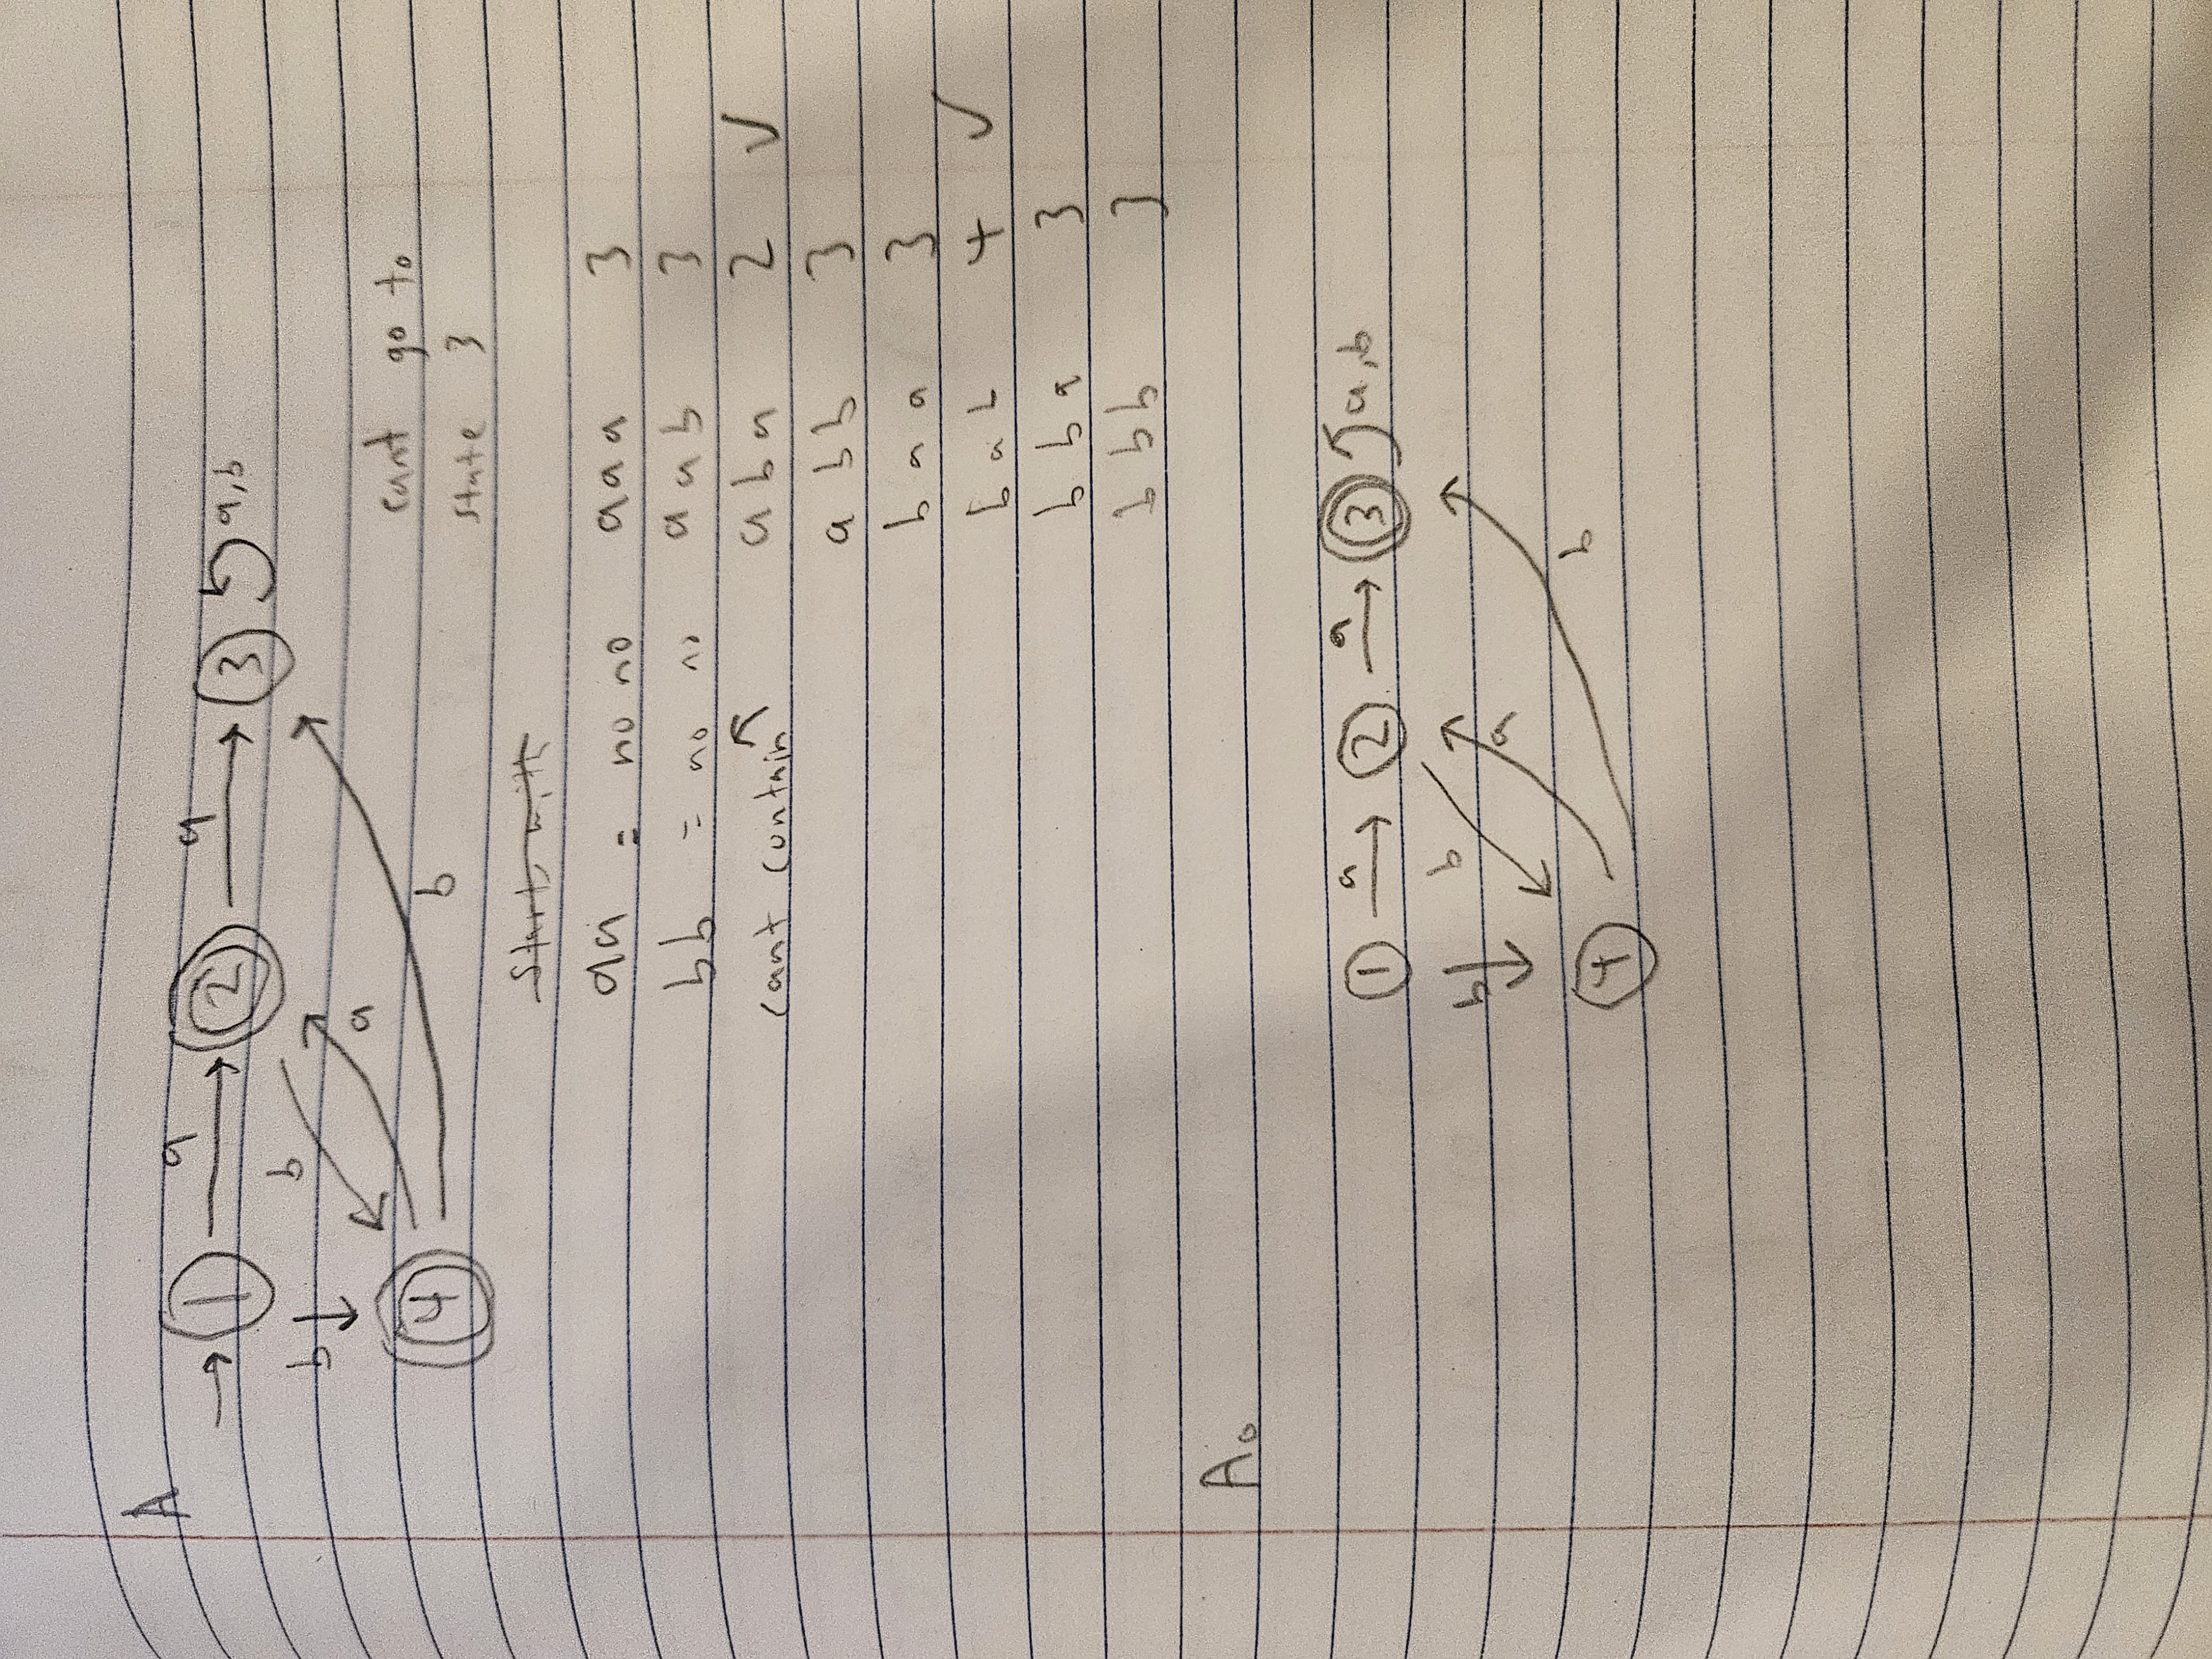
\includegraphics[angle=-90, width=0.7\textwidth]{latexImages/hw2-1.jpg} 
\end{figure}

dfaex03.py (modified)

\begin{lstlisting}[language=Python]
import dfa

def __main__() :

    Q1 = {1, 2, 3, 4}
    Sigma1 = ['a', 'b']
    delta1 = {
        (1, 'a'): 2,
        (1, 'b'): 4,
        (2, 'a'): 3,
        (2, 'b'): 4,
        (3, 'a'): 3,
        (3, 'b'): 3,
        (4, 'a'): 2,
        (4, 'b'): 3,
    }
    q0_1 = 1
    F1 = {2, 4}  
    A = dfa.DFA(Q1, Sigma1, delta1, q0_1, F1)

    Q2 = {1, 2, 3, 4}
    Sigma2 = ['a', 'b']
    delta2 = {
        (1, 'a'): 2,
        (1, 'b'): 4,
        (2, 'a'): 3,
        (2, 'b'): 4,
        (3, 'a'): 3,
        (3, 'b'): 3,
        (4, 'a'): 2,
        (4, 'b'): 3,
    }
    q0_2 = 1
    F2 = {3}  # Only state 3 is accepting
    A1 = dfa.DFA(Q2, Sigma2, delta2, q0_2, F2)
    #A1 should be equivalent to A0 if tests are correct
    #all that I did was swap the final, non initial states with non-final
    #non starting states, meaning in this case all that changes
    #is F containing 3 instead of 2, 4
    
    #testWord1 should be accepted by A and refused by A0
    #testWord2 should be accepted by A0 and refused by A
    testWords1 = ["aabababa", "ababaab", "bbaababaa"]
    testWords2 = ["ababa", "bababa", "ababababab"]

    A0 = A.refuse()

    testAutomata = [A, A1, A0]
    print("Test words 1\n")
    for automata in testAutomata:
        print(f"{automata.__repr__()}")
        for w in testWords1:
            print(f"{w}: {automata.run(w)}")
        print("\n")
    
    print("Test words 2\n")
    for automata in testAutomata:
        print(f"{automata.__repr__()}")
        for w in testWords2:
            print(f"{w}: {automata.run(w)}")
        print("\n")
        
__main__()
\end{lstlisting}

The modifications made to dfa.py were to add the run and refuse methods.  The run method works by essentially telling us the next
state that would be in after the last symbol is seen by the function.  So for A1, if 2 is the last state seen, and the incoming symbol is b, then the final state returned will be state 3.

In the refuse method works on an instance of the DFA object that calls it,  I start with an empty set of states,  and iterate over the set of all states of the DFA.  Then,  that state is appended to the empty set of states as the function checks if the states in the set F of final states.  Basically,  the goal to make the compliment of A was to swap the middle states with final states, meaning the opposite words are accepted.

\subsubsection{Exercise 2.2.4}


\begin{enumerate}
    \item 
    \begin{multline*}
        L_1 = \{ w \mid w \text{ ends with } 00, \text{ where } w = x00, \\
        \text{for some string } x \text{ consisting of only 0's and 1's} \}
    \end{multline*}

    \item 
    \begin{multline*}
        L_2 = \{ w \mid w \text{ contains } 000 \text{ as a substring, meaning } \\
        w = x000y, 000y, \text{ or } x000, \text{ where } x, y \text{ are strings} \\
        \text{consisting of only 0's and 1's} \}
    \end{multline*}

    \item 
    \begin{multline*}
        L_3 = \{ w \mid w \text{ contains } 011 \text{ as a substring, meaning } \\
        w = x011y, \text{ where } x, y \text{ are strings consisting of only 0's and 1's} \}
    \end{multline*}
\end{enumerate}

Question: Aside from tables and diagrams, could there be another niche method of representing DFAs that would be useful for some purpose?

\subsection{HW 3}

\subsubsection{Operations on automata: homework 1 and 2}

\begin{figure}[H]
    \centering
    \includegraphics[angle=-90, width=0.7\textwidth]{latexImages/hw3-1.1.jpg} 
\end{figure}

\begin{figure}[H]
    \centering
    \includegraphics[angle=-90, width=0.7\textwidth]{latexImages/hw3-1.2.jpg} 
\end{figure}

\subsubsection{Exercise 2.2.7}
\begin{figure}[H]
    \centering
    \includegraphics[angle=-90, width=0.7\textwidth]{latexImages/hw3-2.jpg} 
\end{figure}

Question: Can two different NFAs recognize the same language but process words in fundamentally different ways?

\subsection{HW 4}

\subsubsection{Determinization: homework 1 and 2}

\begin{figure}[H]
    \centering
    \includegraphics[angle=-90, width=0.7\textwidth]{latexImages/hw4-1.1.jpg} 
\end{figure}

\begin{figure}[H]
    \centering
    \includegraphics[angle=-90, width=0.7\textwidth]{latexImages/hw4-2.1.jpg} 
\end{figure}

\begin{figure}[H]
    \centering
    \includegraphics[angle=-90, width=0.7\textwidth]{latexImages/hw4-2.2.jpg} 
\end{figure}

\begin{figure}[H]
    \centering
    \includegraphics[angle=-90, width=0.7\textwidth]{latexImages/hw4-2.3.jpg} 
\end{figure}

\begin{figure}[H]
    \centering
    \includegraphics[angle=-90, width=0.7\textwidth]{latexImages/hw4-2.4.jpg} 
\end{figure}

Question: What patterns can we observe in potential real world applications for automata that indicate strongly or weakly which type of automatom is most useful?

\subsection{HW 5}

\subsubsection{Exercise 3.2.1}

\begin{figure}[H]
    \centering
    \includegraphics[angle=-90, width=0.7\textwidth]{latexImages/hw5-3.2.1.jpg} 
\end{figure}

\begin{figure}[H]
    \centering
    \includegraphics[angle=0, width=0.9\textwidth]{latexImages/hw5-3.2.1-d.jpg} 
\end{figure}

\subsubsection{Exercise 3.2.2}

\begin{figure}[H]
    \centering
    \includegraphics[angle=-90, width=0.7\textwidth]{latexImages/hw5-3.2.2.jpg} 
\end{figure}

\subsubsection{Exercise 4.4.1}

\begin{figure}[H]
    \centering
    \includegraphics[angle=-90, width=0.7\textwidth]{latexImages/hw5-4.4.1.jpg} 
\end{figure}

\begin{figure}[H]
    \centering
    \includegraphics[angle=-90, width=0.7\textwidth]{latexImages/hw5-4.4.1-b.jpg} 
\end{figure}

\subsubsection{Exercise 4.4.2}

\begin{figure}[H]
    \centering
    \includegraphics[angle=-90, width=0.7\textwidth]{latexImages/hw5-4.4.2.jpg} 
\end{figure}

Question: Is there a more compact way to display the same information as in a filling table once an automata reaches a certain size , or are other methods better/worse at being compact depending on number of accepting states or other variables?

\section{Synthesis}

\section{Evidence of Participation}

\section{Conclusion}\label{conclusion}


\begin{thebibliography}{99}
    \bibitem[BLA]{bla} Author, \href{https://en.wikipedia.org/wiki/LaTeX}{Title}, Publisher, Year.
    \end{thebibliography}

\end{document}